\chapter{Antecedentes y justificación}
\thispagestyle{fancy}
\fancyhead[LE]{\thechapter.Antecedentes y justificación}

\section{Antecedentes}


\subsection{Sistemas de recomendación}
Los sistemas de recomendación fueron mencionados por primera vez en los años 90 y han ido evolucionando hasta estar implantados en gran parte de las empresas actuales. Estos sistemas son sistemas de filtrado de información, que se basan en una gran cantidad de datos, tanto del usuario como de los elementos a recomendar, para predecir cuál será el elemento más apropiado para este. Estos sistemas están estrechamente relacionados con el marketing, ya que el objetivo es conseguir recomendar un elemento que sea del agrado e interés del usuario con los datos que se tienen de él, lo que en la mayoría de los casos va ligado al consumo de bienes o servicios. 
\\ \\
Hoy en día se usan en multitud de ámbitos, desde las redes sociales hasta las distribuidoras de contenido como Netflix, pasando por compañías de comercio electrónico como Amazon. 
\\ \\
A la hora de realizar la recomendación se realizan filtrados de diferente tipo, estos no son más que la forma en la que el sistema busca correlacionar los usuarios con los elementos que estos consumen, compran o ven. Entre los métodos más comunes para relacionar esta información y obtener resultados eficientes se encuentran:
\begin{itemize}
    \item Filtros demográficos, que recomiendan en función del sexo, edad, país, oficio, … 
    \item Filtros basados en contenidos, como Youtube, que recomiendan contenidos similares a los valorados por los usuarios. 
    \item Filtrado colaborativo, que consiste en recomendar al usuario elementos valorados positivamente por usuarios similares a él. 
\end{itemize}

Sin embargo, existen sistemas híbridos que utilizan varias de las estrategias de filtrado anteriores combinadas. Un ejemplo de ello es el mencionado Amazon, que tiene uno de los algoritmos de recomendación más potentes y eficientes actualmente. 
\\ \\
Sin embargo, existen sistemas híbridos que utilizan varias de las estrategias de filtrado anteriores combinadas. Un ejemplo de ello es el mencionado Amazon, que tiene uno de los algoritmos de recomendación más potentes y eficientes actualmente. 
\\ \\
Esto se debe a dos cosas, en primer lugar que cuenta con una gran cantidad de información de los usuarios, tanto su edad, género, país, dirección, rutinas (si tienen Alexa), … como los artículos que miran, compran, añaden a la lista, etc. Con todo esto el algoritmo es capaz de ofrecer recomendaciones muy precisas a los usuarios, lo que le da una gran calidad de servicio a la empresa gracias a esto.
\\ \\
De hecho, en Amazon, si queremos revisar las recomendaciones tenemos un apartado propio para ellas al que se puede acceder fácilmente (Fig\ref{fig:AmazonRecomendaciones}).
\begin{figure}[thbp]
    \centering
    \fbox{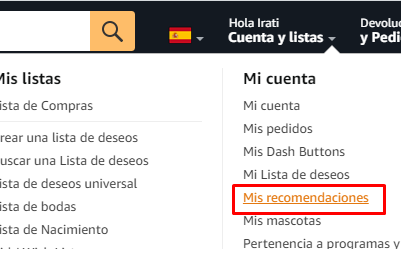
\includegraphics[width=0.45\textwidth]{Figuras/Amazon_acceder_mis_recomendaciones.png}}
    \fbox{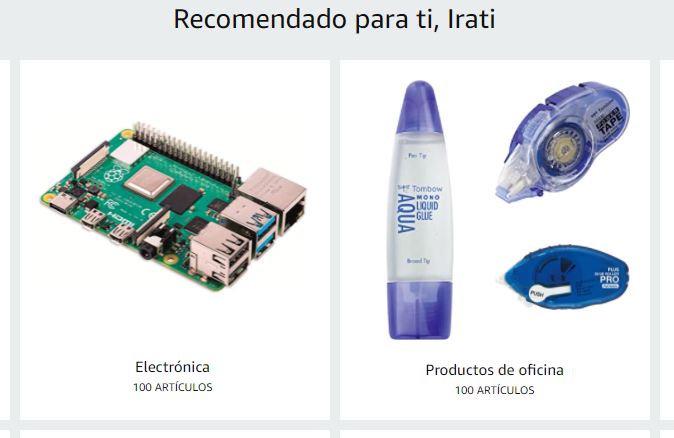
\includegraphics[width=0.45\textwidth]{Figuras/Amazon_recomendaciones.png}}
    \caption{Recomendaciones de Amazon (Fuente: Amazon\autocite{AmazonEsCompra})} 
    \label{fig:AmazonRecomendaciones}
\end{figure}